\documentclass{article}
\usepackage{graphicx} %package to manage images
\usepackage[utf8]{inputenc}
\usepackage[a4paper, total={6in, 8in}]{geometry}
\usepackage{xurl}
\usepackage{hyperref}
\usepackage{float}
\title{Relatório 6 \\ Matching}
\author{Pedro A. S. O. Neto}
\date{Junho, 2023}

\begin{document}

\maketitle

\section{Matching between samples}

There were notable discrepancies in age between our original samples of TD and TEA participants (Table 1). Additionally, there was a significant gender(?) imbalance, with 47\% of females in the TD group, and only 6\% in amongst TEA participants.

To address this issue, we employed a matching algorithm suggested by Ho, Imai, King \& Stuart (2011), which minimized the Euclidean distance based on participants' sex and age. Following the matching process, our final sample consisted of 15 participants from each diagnostic group (refer to Table X for descriptive statistics).

\begin{table}[H]
\parbox{.45\linewidth}{
\centering
\begin{tabular}{cccc}
\hline
    tea & meanAge & sdAge & N \\ 
    \hline
    TD & 2.87 & 1.04 & 358 \\ 
    TEA & 3.06 & 0.79 &  15 \\ 
\hline
\end{tabular}
\caption{Non matched}
}
\hfill
\parbox{.45\linewidth}{
\centering
\begin{tabular}{cccc}
\hline
   tea & meanAge & sdAge & N  \\ 
    \hline
    TD & 3.05 & 0.78 &  15 \\ 
    TEA & 3.06 & 0.79 & 15 \\ 
\hline
\end{tabular}
\caption{Matched}
}
\end{table}


\section{ANOVA}

Same analysis as report 5, but with matched samples. Main effects and interaction were the same between matched and unmatched samples.


\subsection{Alternancias}

\begin{table}[H]
\centering
\caption{Alternancias}
\begin{tabular}{lrrrrrr}
  \hline
 & Df & Sum Sq & Mean Sq & F value & Pr($>$F) & \\ 
  \hline
  condition              & 1 & 2.30 & 2.30 & 8.71 & 0.0035 & **\\ 
  tea                    & 1 & 1.68 & 1.68 & 6.37 & 0.0123 & *\\ 
  variable               & 3 & 25.16 & 8.39 & 31.80 & 0.00 & ***\\ 
  condition:tea          & 1 & 0.01 & 0.01 & 0.02 & 0.8809 & \\ 
  condition:variable     & 3 & 4.89 & 1.63 & 6.17 & 0.0005 & ***\\ 
  tea:variable           & 3 & 0.43 & 0.14 & 0.54 & 0.6544 & \\ 
  condition:tea:variable & 3 & 0.30 & 0.10 & 0.38 & 0.7711 & \\ 
  Residuals              & 224 & 59.09 & 0.26 &  &  & \\ 
   \hline
\end{tabular}
\end{table}


\begin{figure}[H]
  \caption{Visualizing TEA effect on alternancias. Mean number of alternancias per tea and trial.}
  \noindent\makebox[\textwidth]{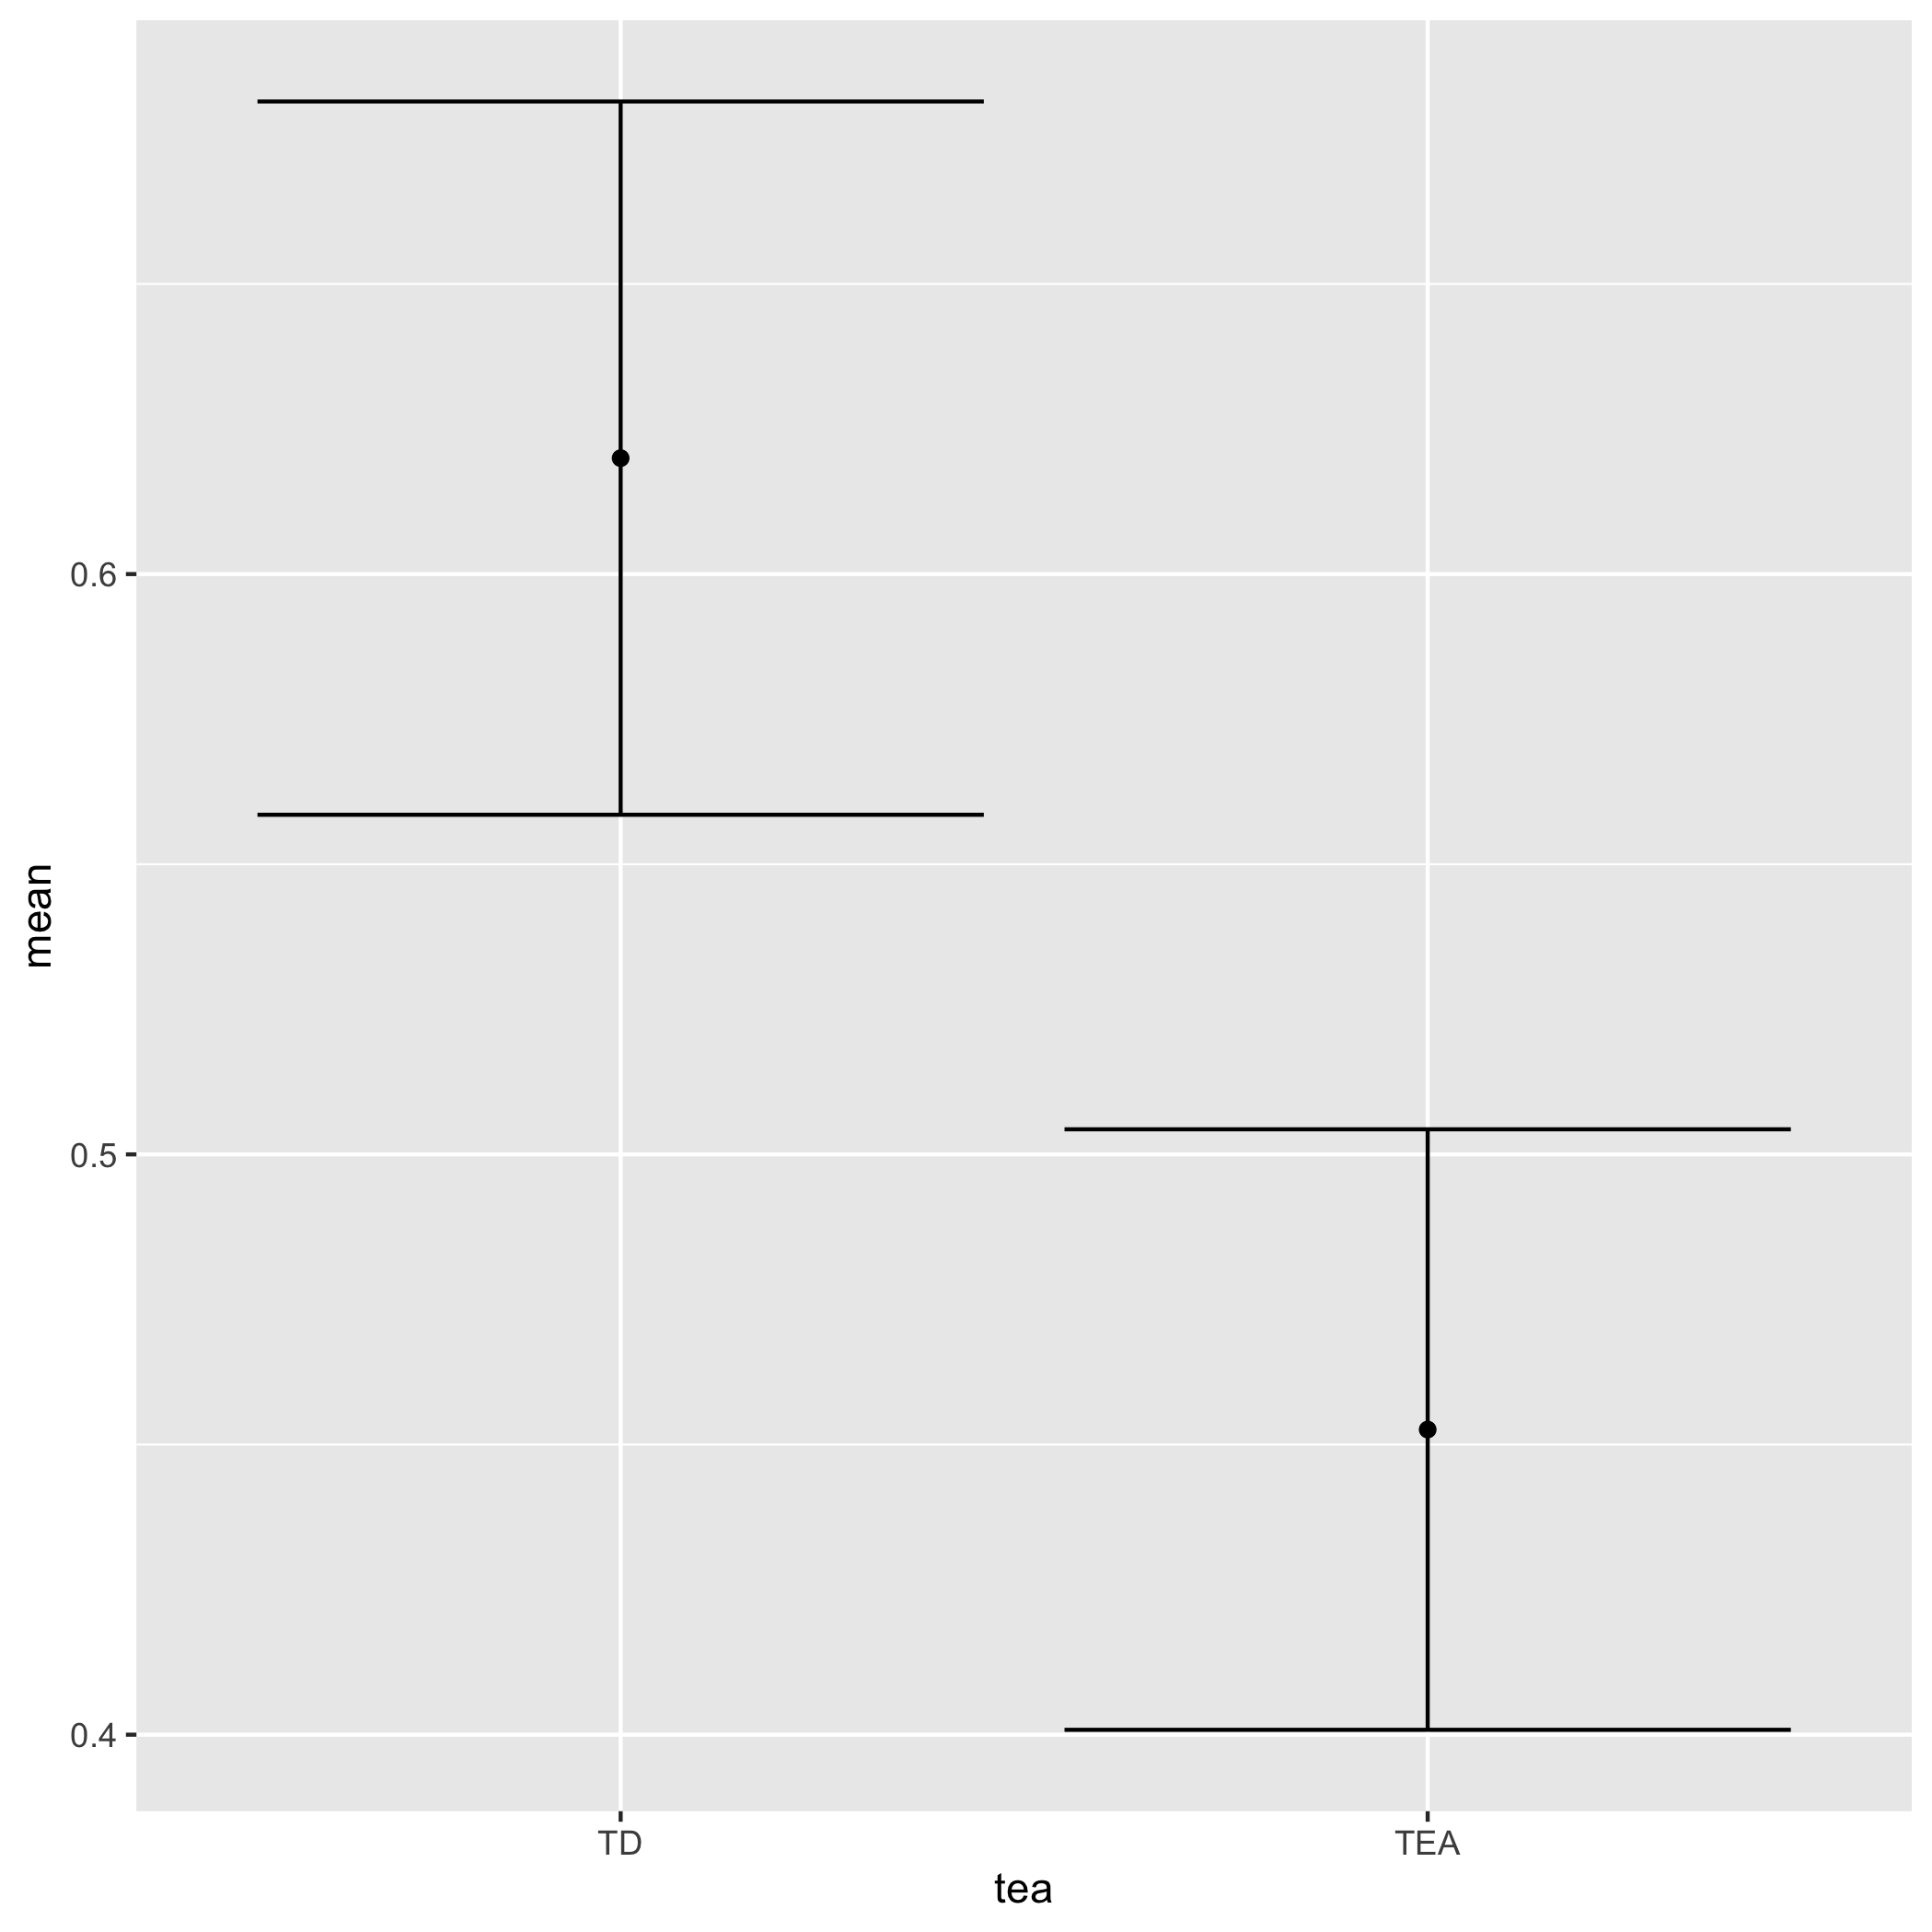
\includegraphics[scale=0.2]{./teaMainAlternancia.png}}
  \centering
\end{figure}

\begin{figure}[H]
  \caption{Visualizing effect of variable}
  \noindent\makebox[\textwidth]{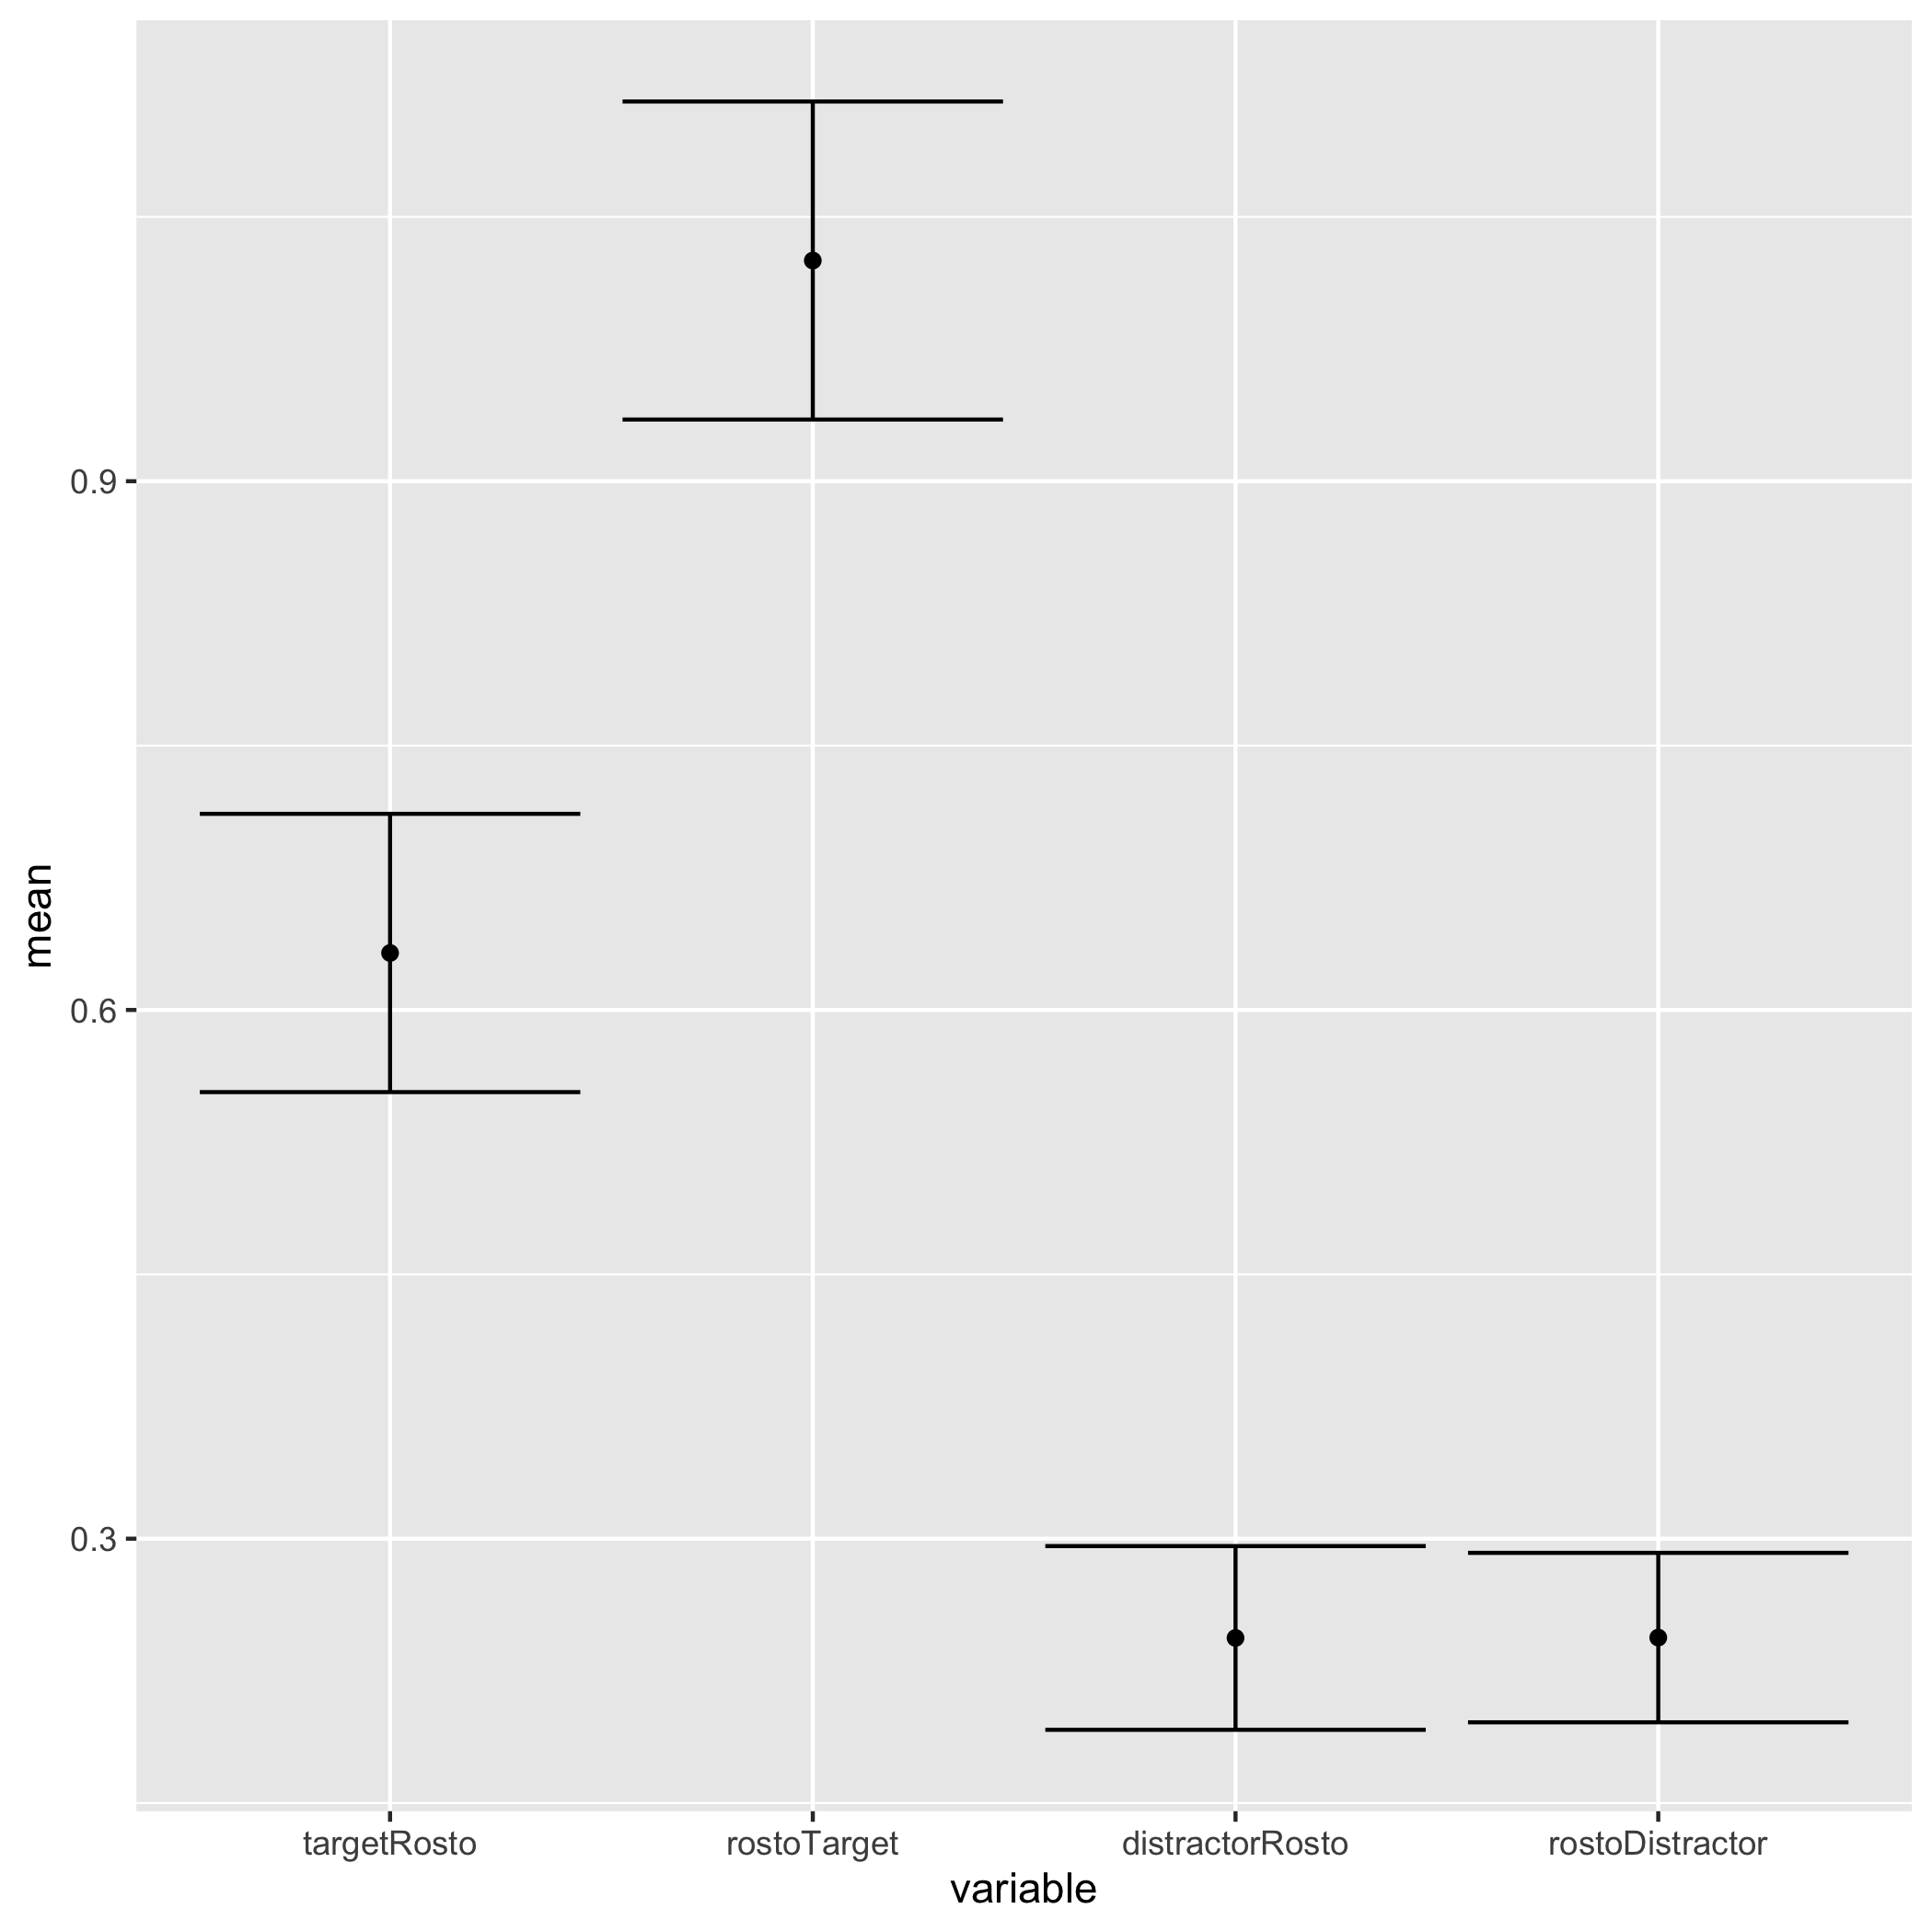
\includegraphics[scale=0.2]{./variableAlternancia.png}}
  \centering
\end{figure}

\begin{figure}[H]
  \caption{Visualizing effect of condition}
  \noindent\makebox[\textwidth]{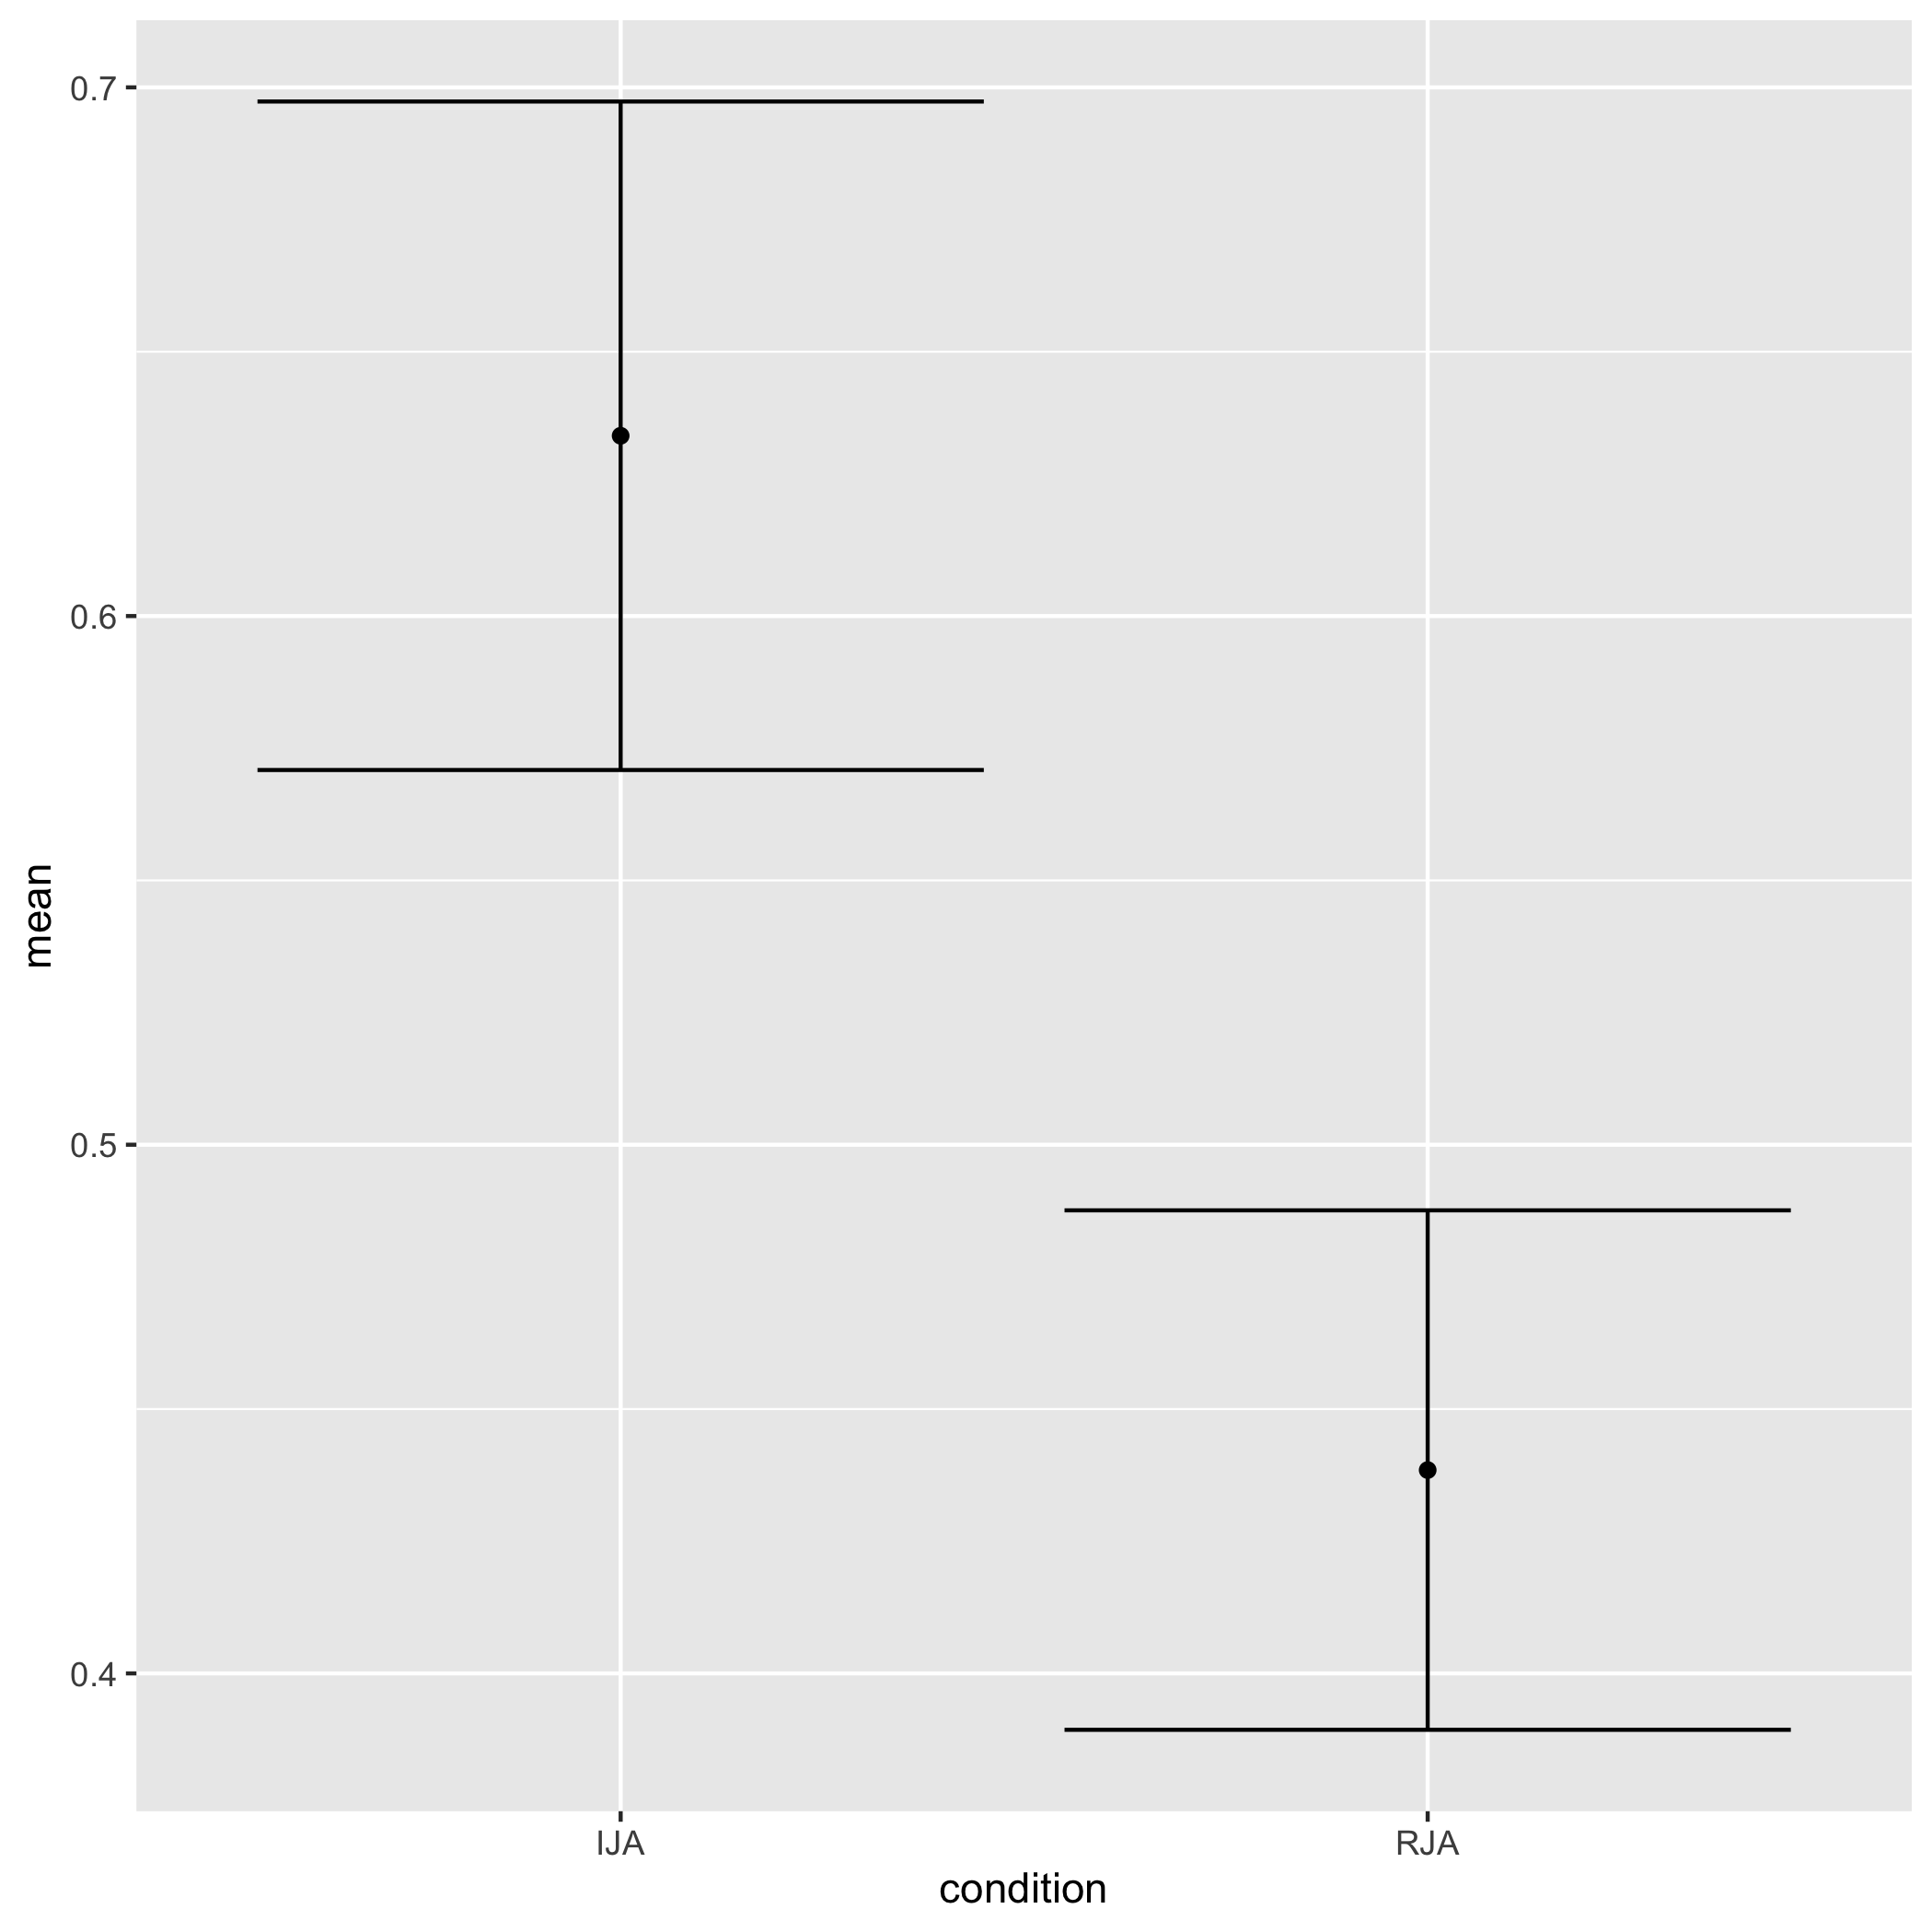
\includegraphics[scale=0.2]{./conditionAlternancia.png}}
  \centering
\end{figure}

\begin{figure}[H]
  \caption{Visualizing interaction of condition and variable}
  \noindent\makebox[\textwidth]{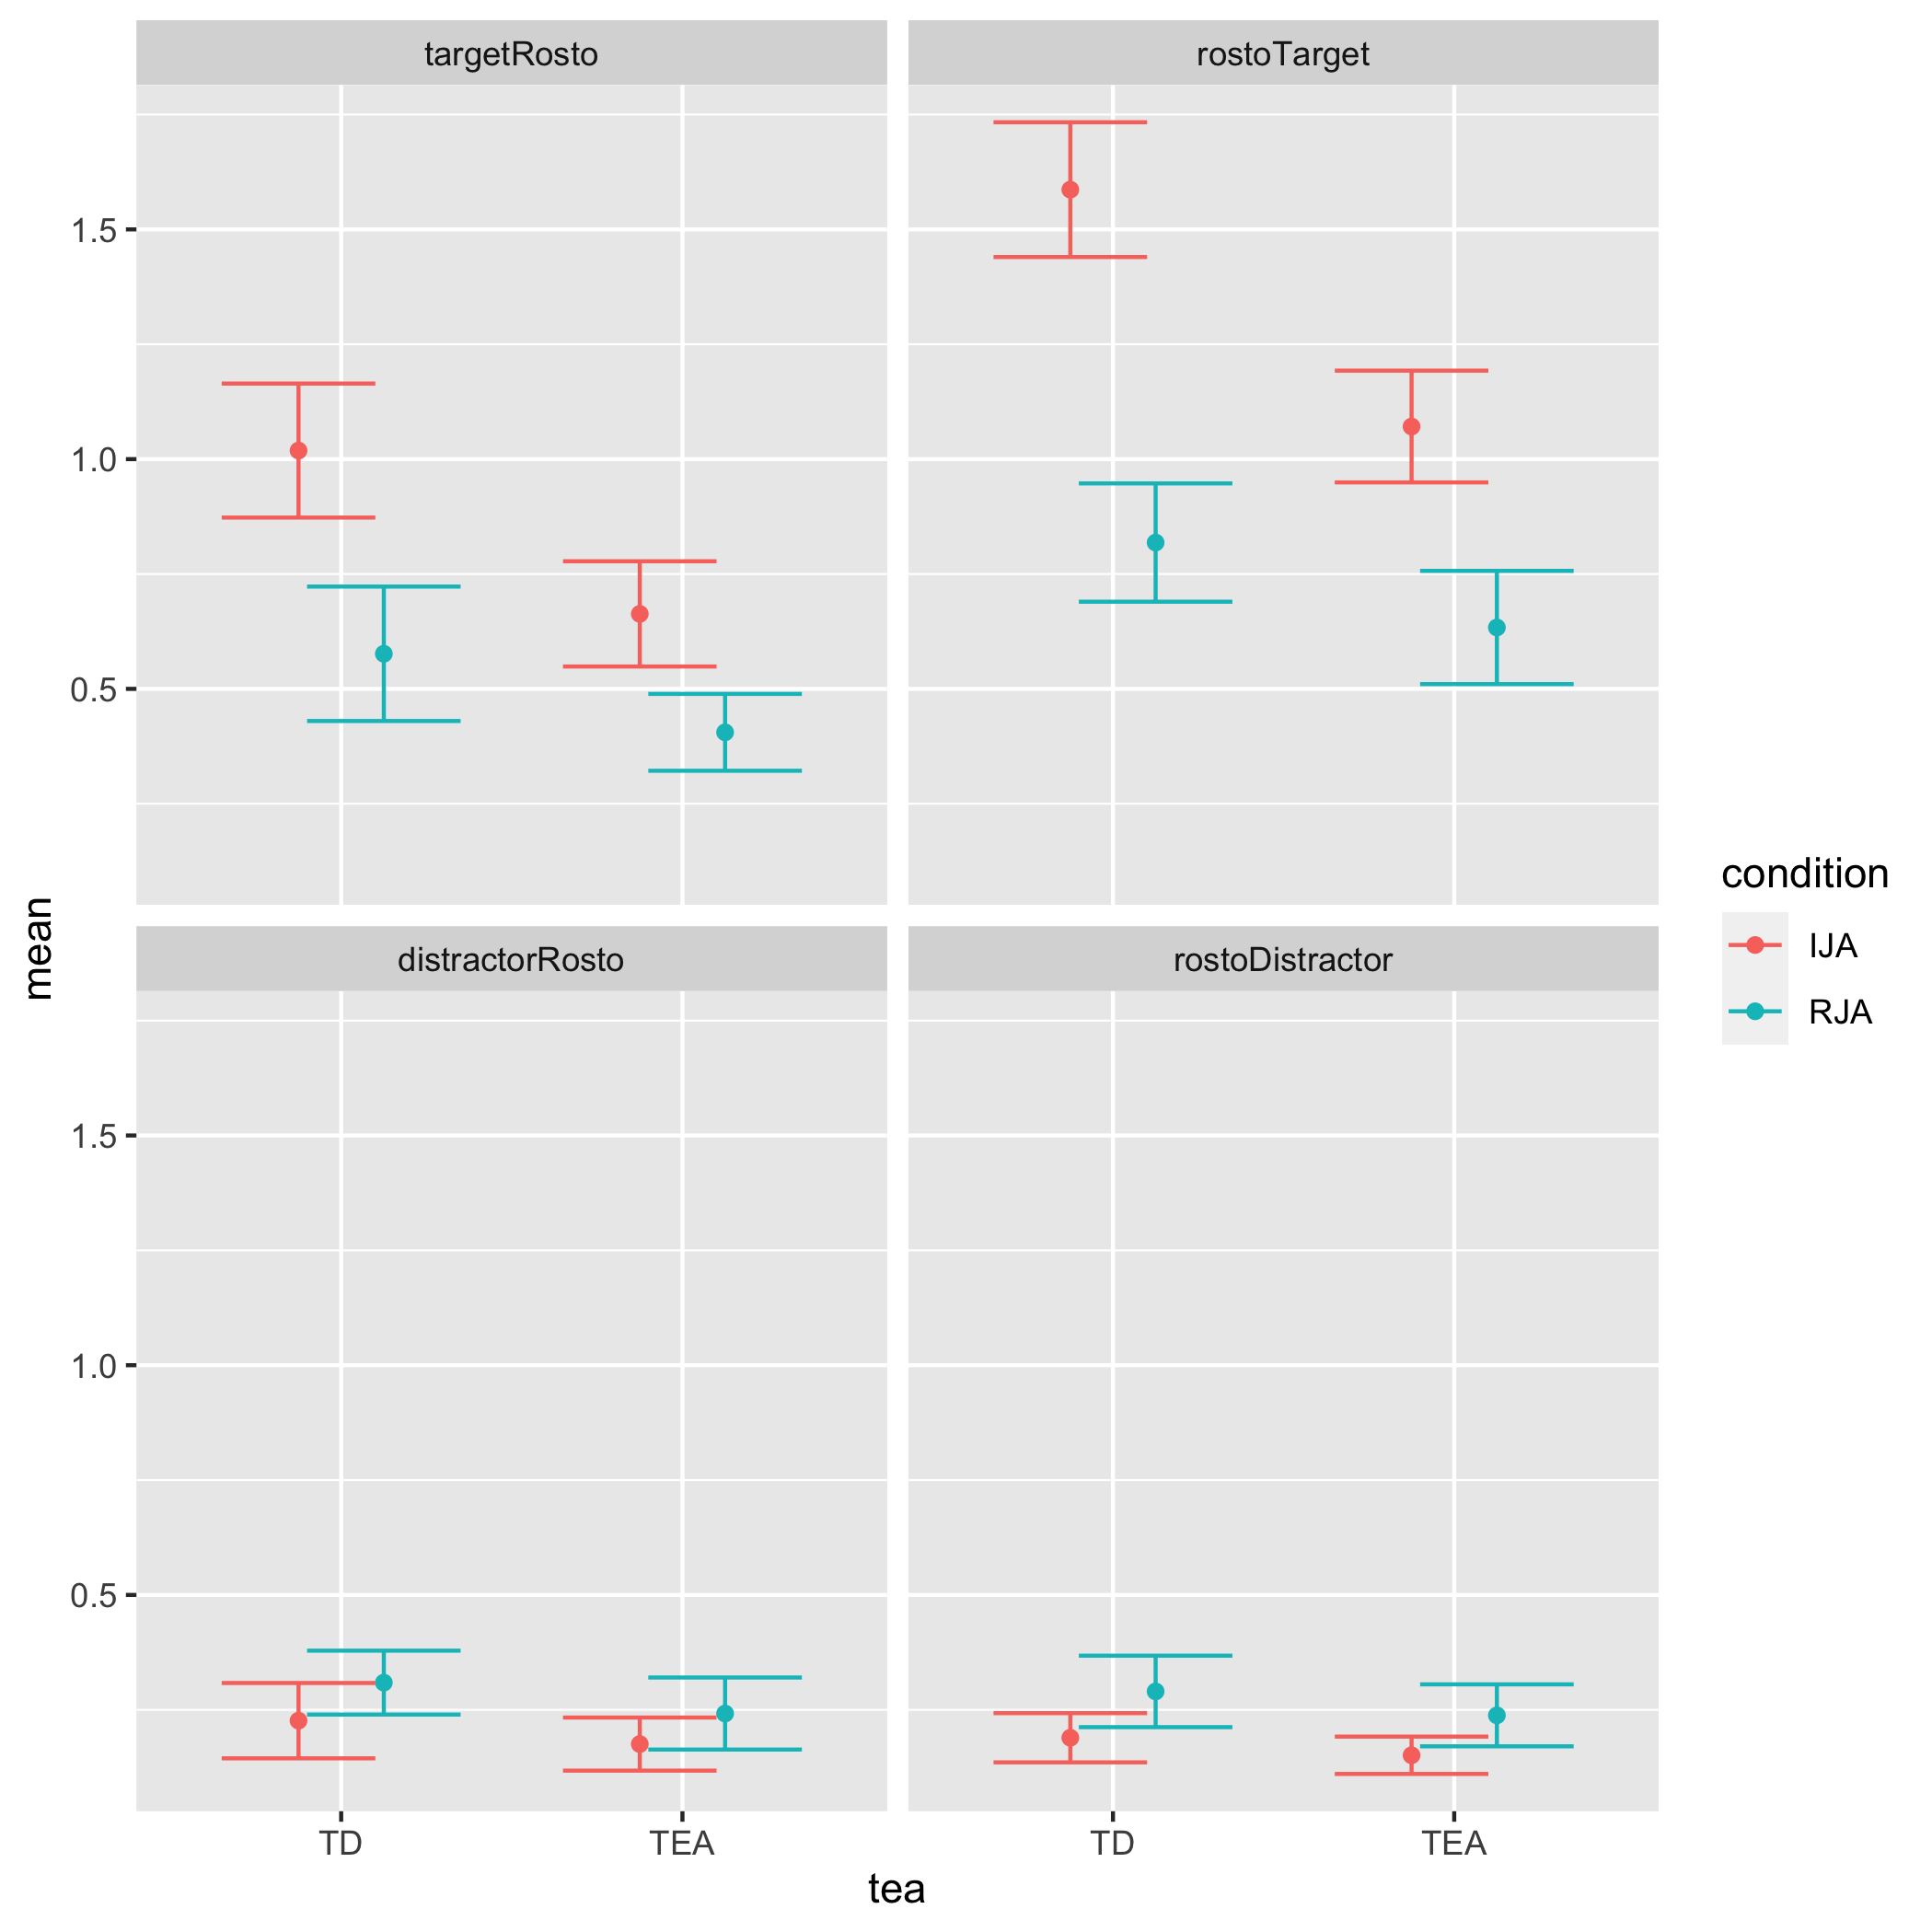
\includegraphics[scale=0.2]{./conditionVariableAlternancia.png}}
  \centering
\end{figure}

\begin{figure}[H]
  \caption{Visualizing interaction between tea and variable}
  \noindent\makebox[\textwidth]{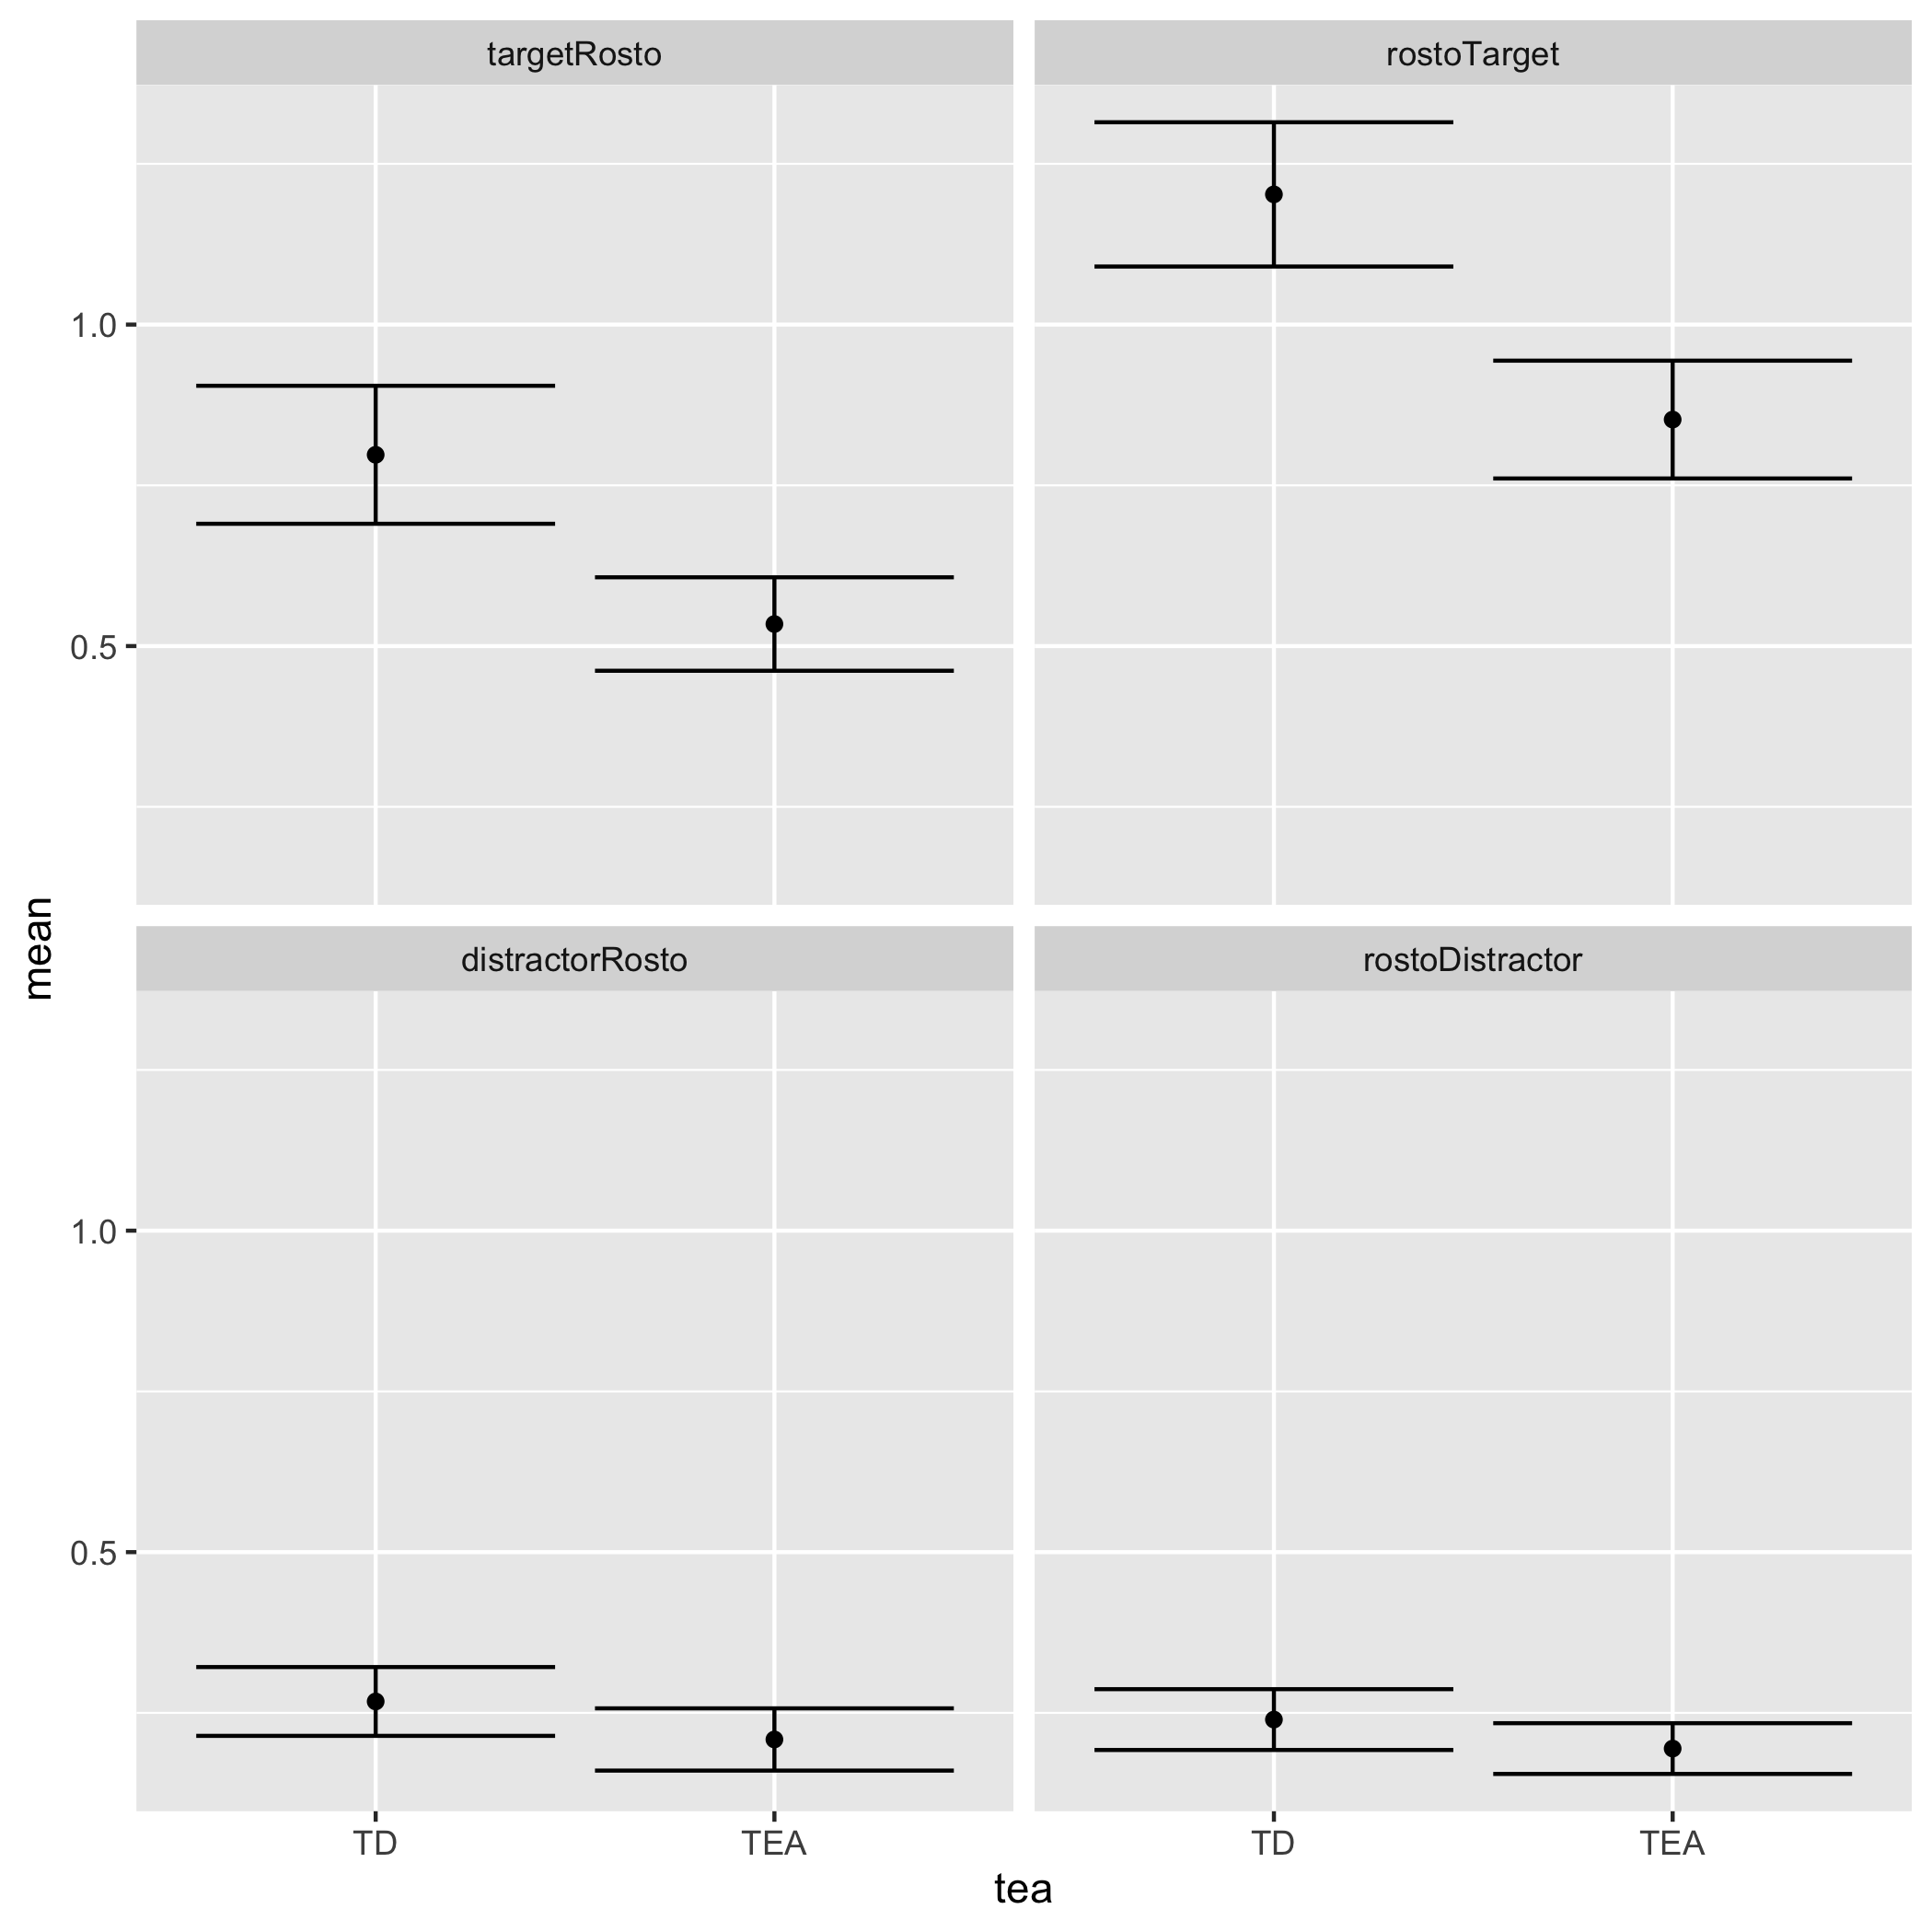
\includegraphics[scale=0.2]{./teaVariableAlternancia.png}}
  \centering
\end{figure}

\subsection{Proportion fixation}

\begin{table}[H]
\centering
\caption{Proportion fixation}
\begin{tabular}{lrrrrrr}
  \hline
 & Df & Sum Sq & Mean Sq & F value & Pr($>$F) & \\ 
  \hline
  condition              & 1 & 0.00 & 0.00 & 0.00 & 1.0000 & \\ 
  tea                    & 1 & 0.00 & 0.00 & 0.00 & 1.0000 & \\ 
  variable               & 3 & 6.37 & 2.12 & 67.56 & 0.0000 & ***\\ 
  condition:tea          & 1 & 0.00 & 0.00 & 0.00 & 1.0000 & \\ 
  condition:variable     & 3 & 1.82 & 0.61 & 19.30 & 0.0000 & ***\\ 
  tea:variable           & 3 & 0.63 & 0.21 & 6.69 & 0.0002 & ***\\ 
  condition:tea:variable & 3 & 0.17 & 0.06 & 1.85 & 0.1387 & \\ 
  Residuals              & 224 & 7.04 & 0.03 &  & & \\ 
   \hline
\end{tabular}
\end{table}

\begin{figure}[H]
  \caption{Visualizing variable effect}
  \noindent\makebox[\textwidth]{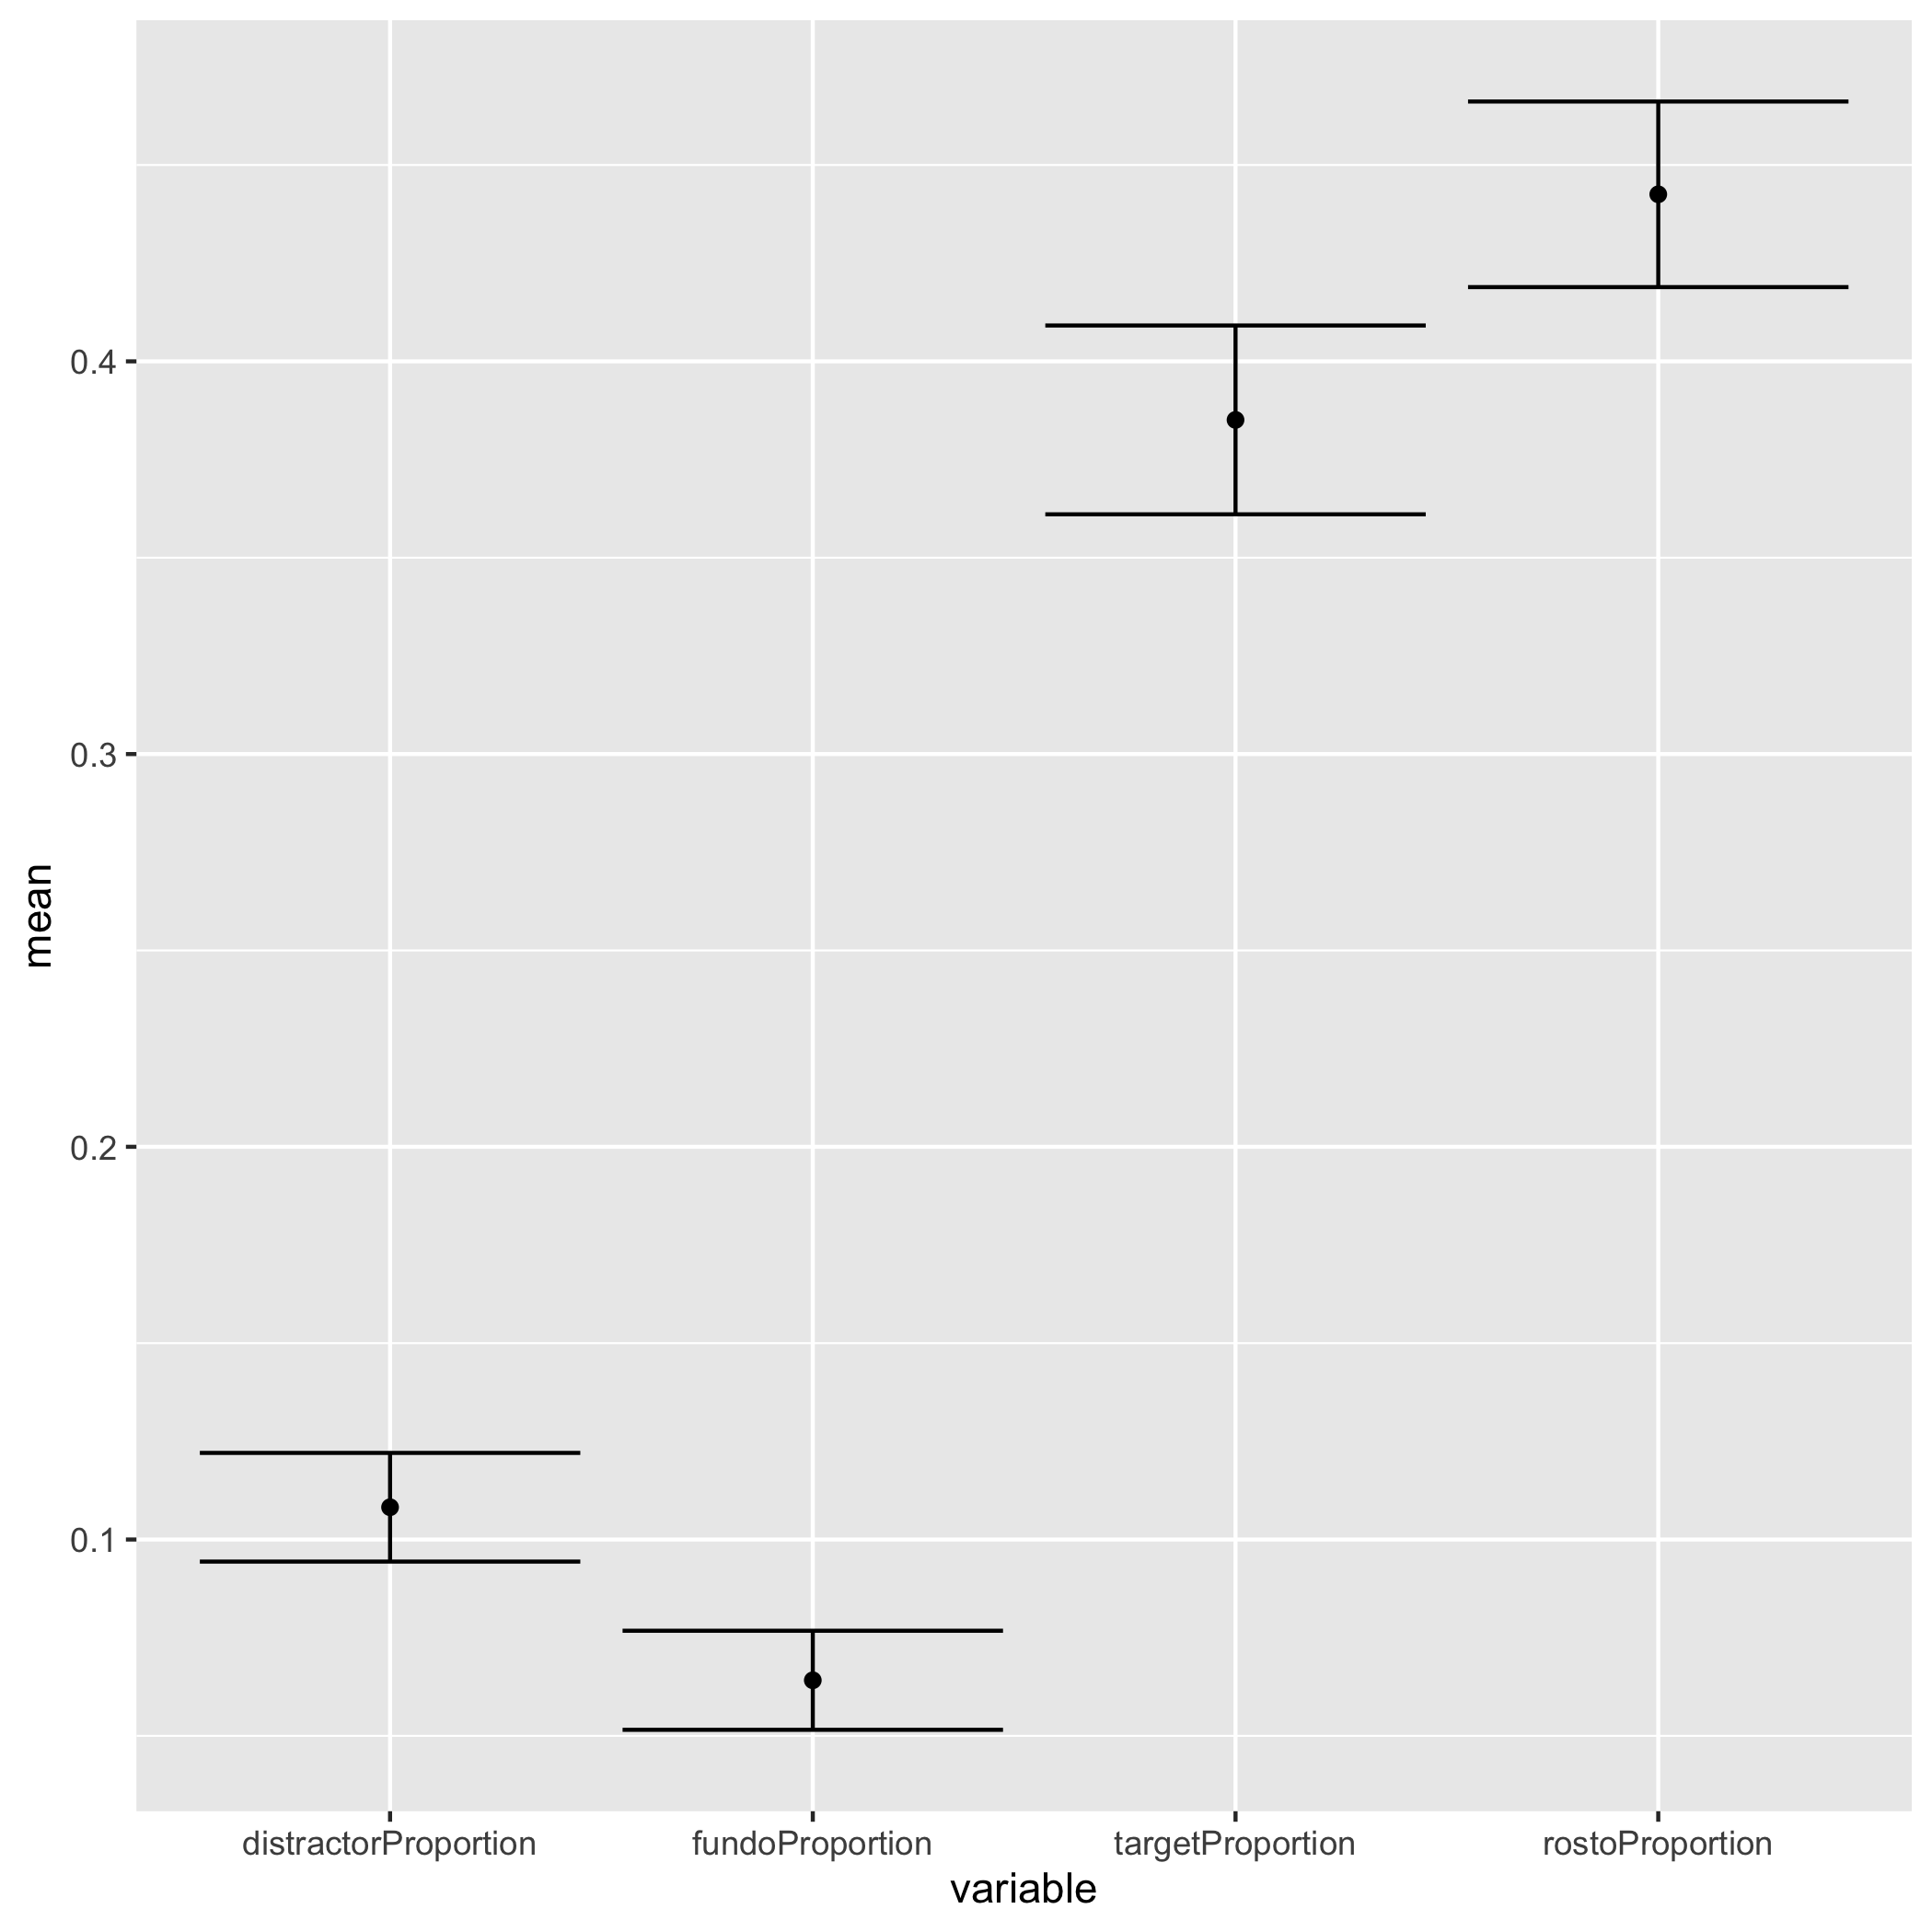
\includegraphics[scale=0.2]{./variableProportion.png}}
  \centering
\end{figure}

\begin{figure}[H]
  \caption{Visualizing interaction condition and variable}
  \noindent\makebox[\textwidth]{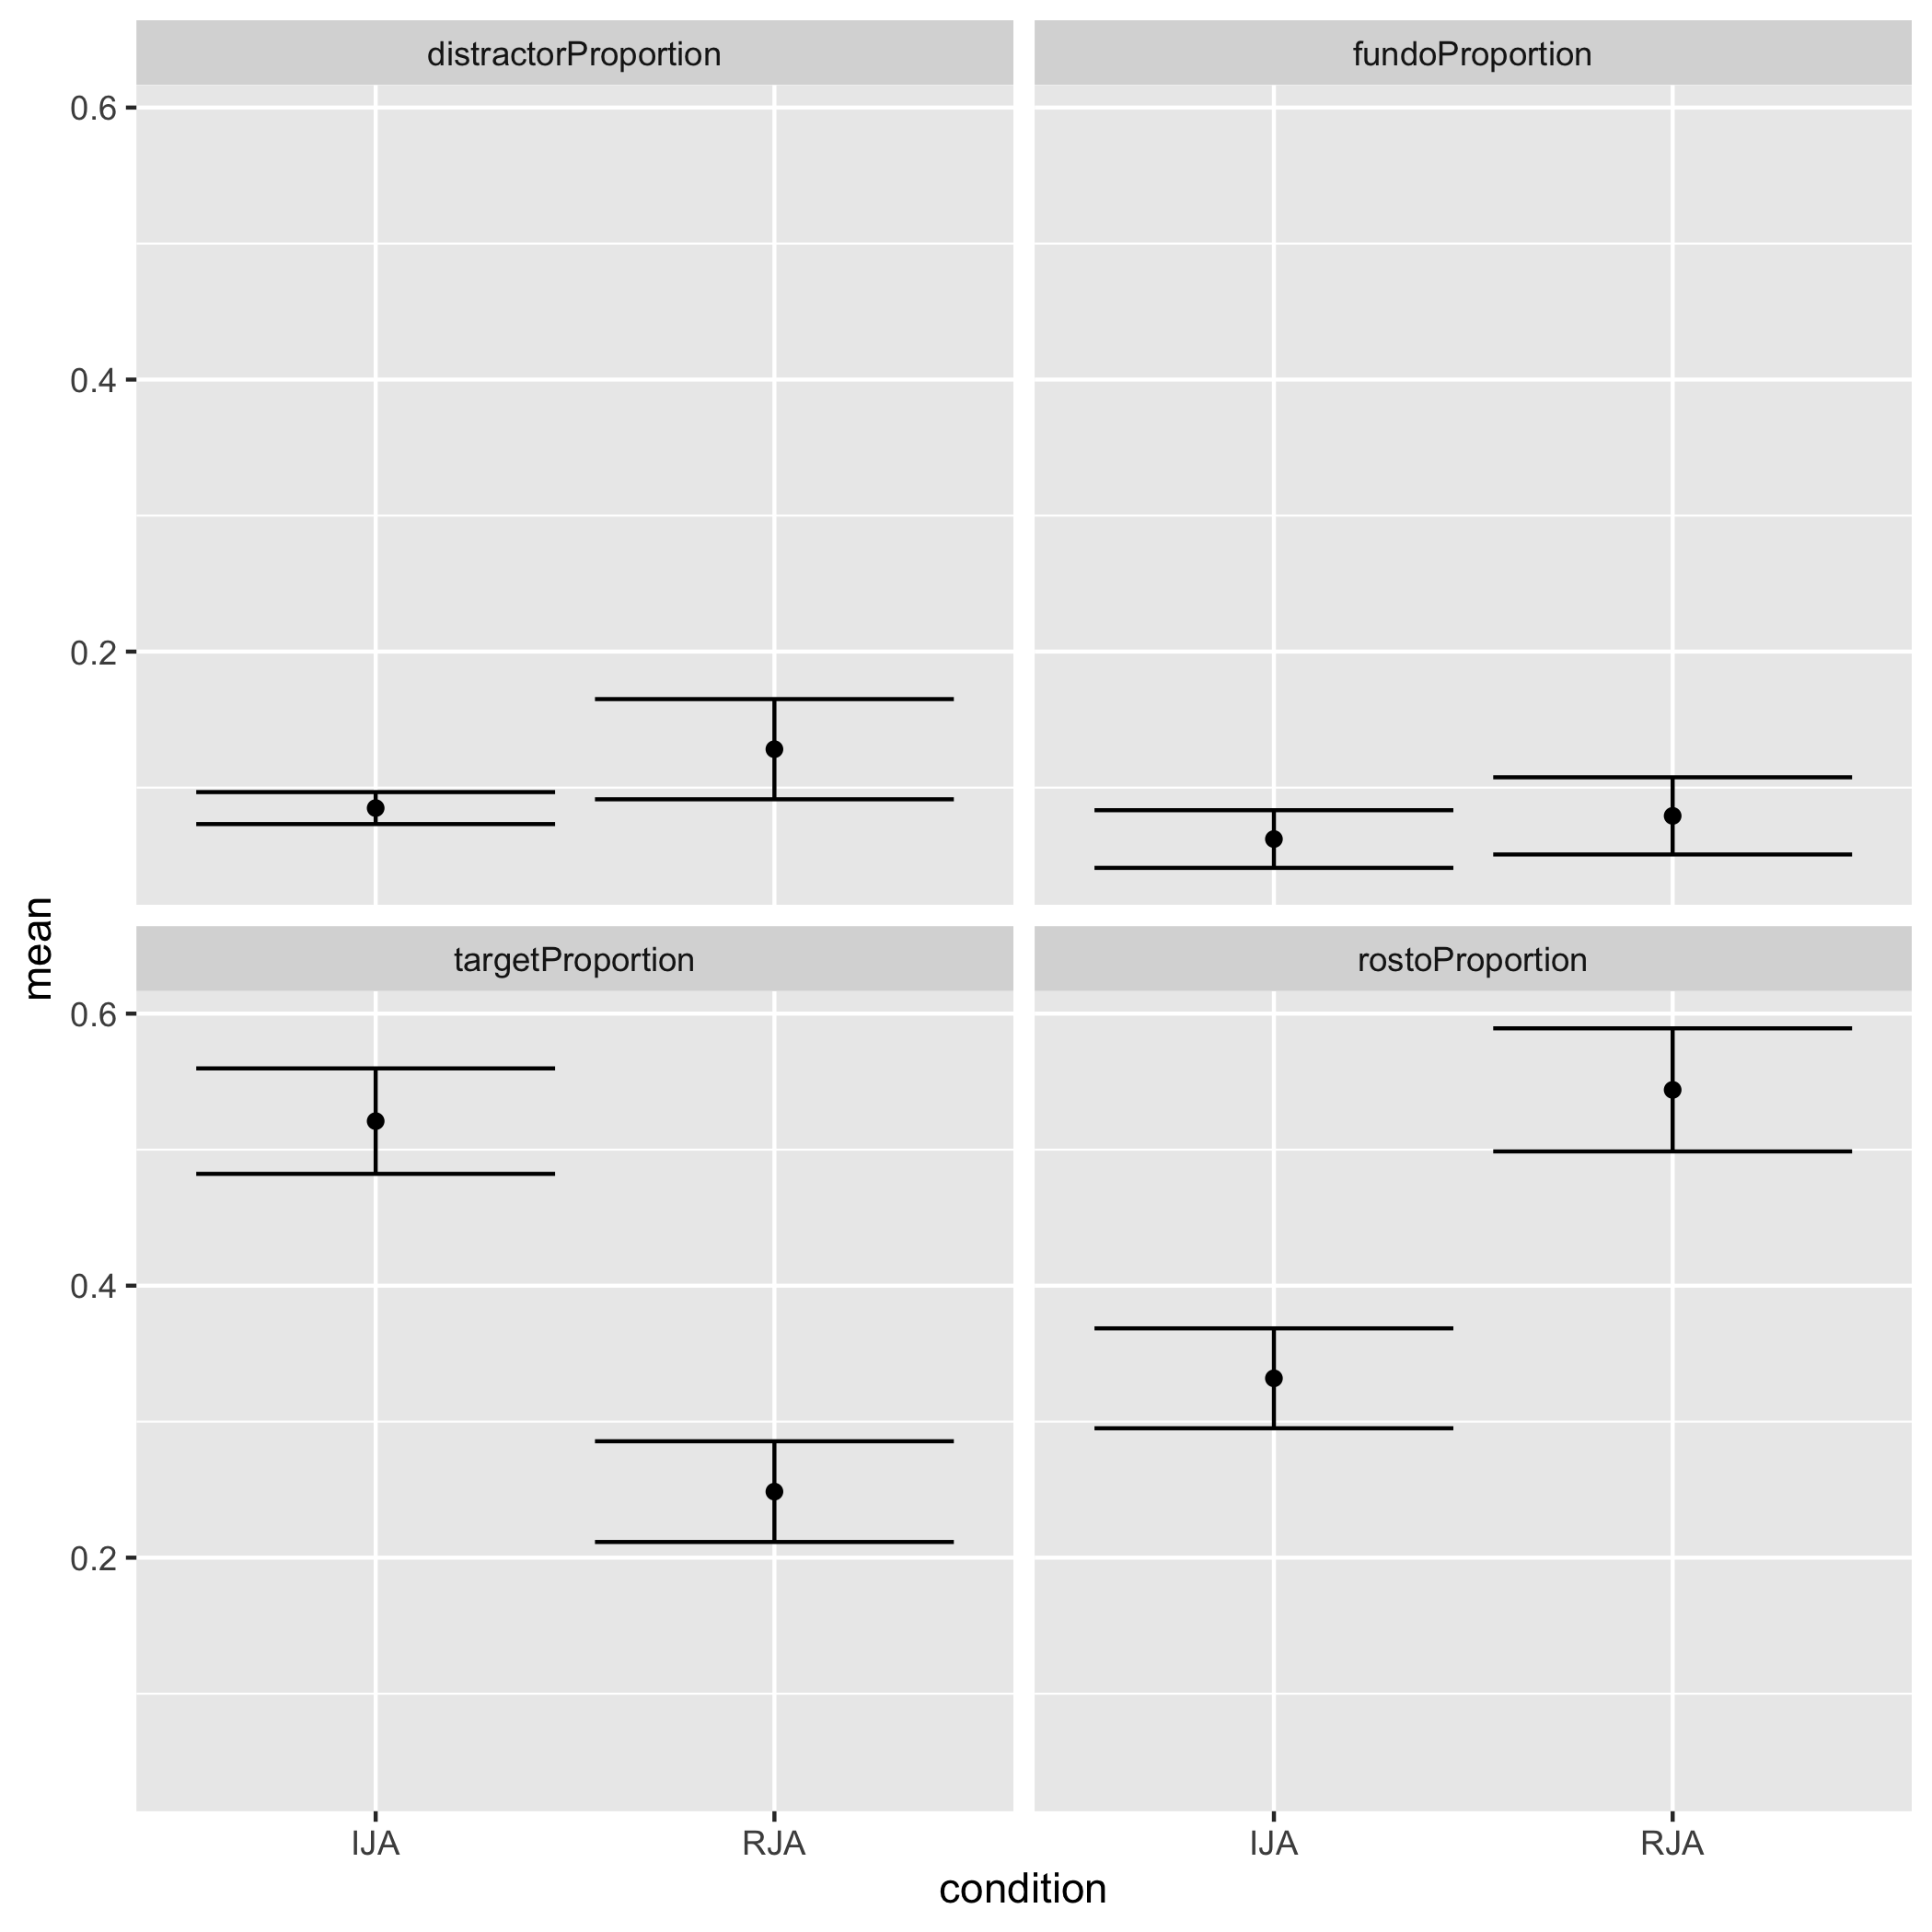
\includegraphics[scale=0.2]{./conditionVariableProportion.png}}
  \centering
\end{figure}

\begin{figure}[H]
  \caption{Visualizing interaction tea variable}
  \noindent\makebox[\textwidth]{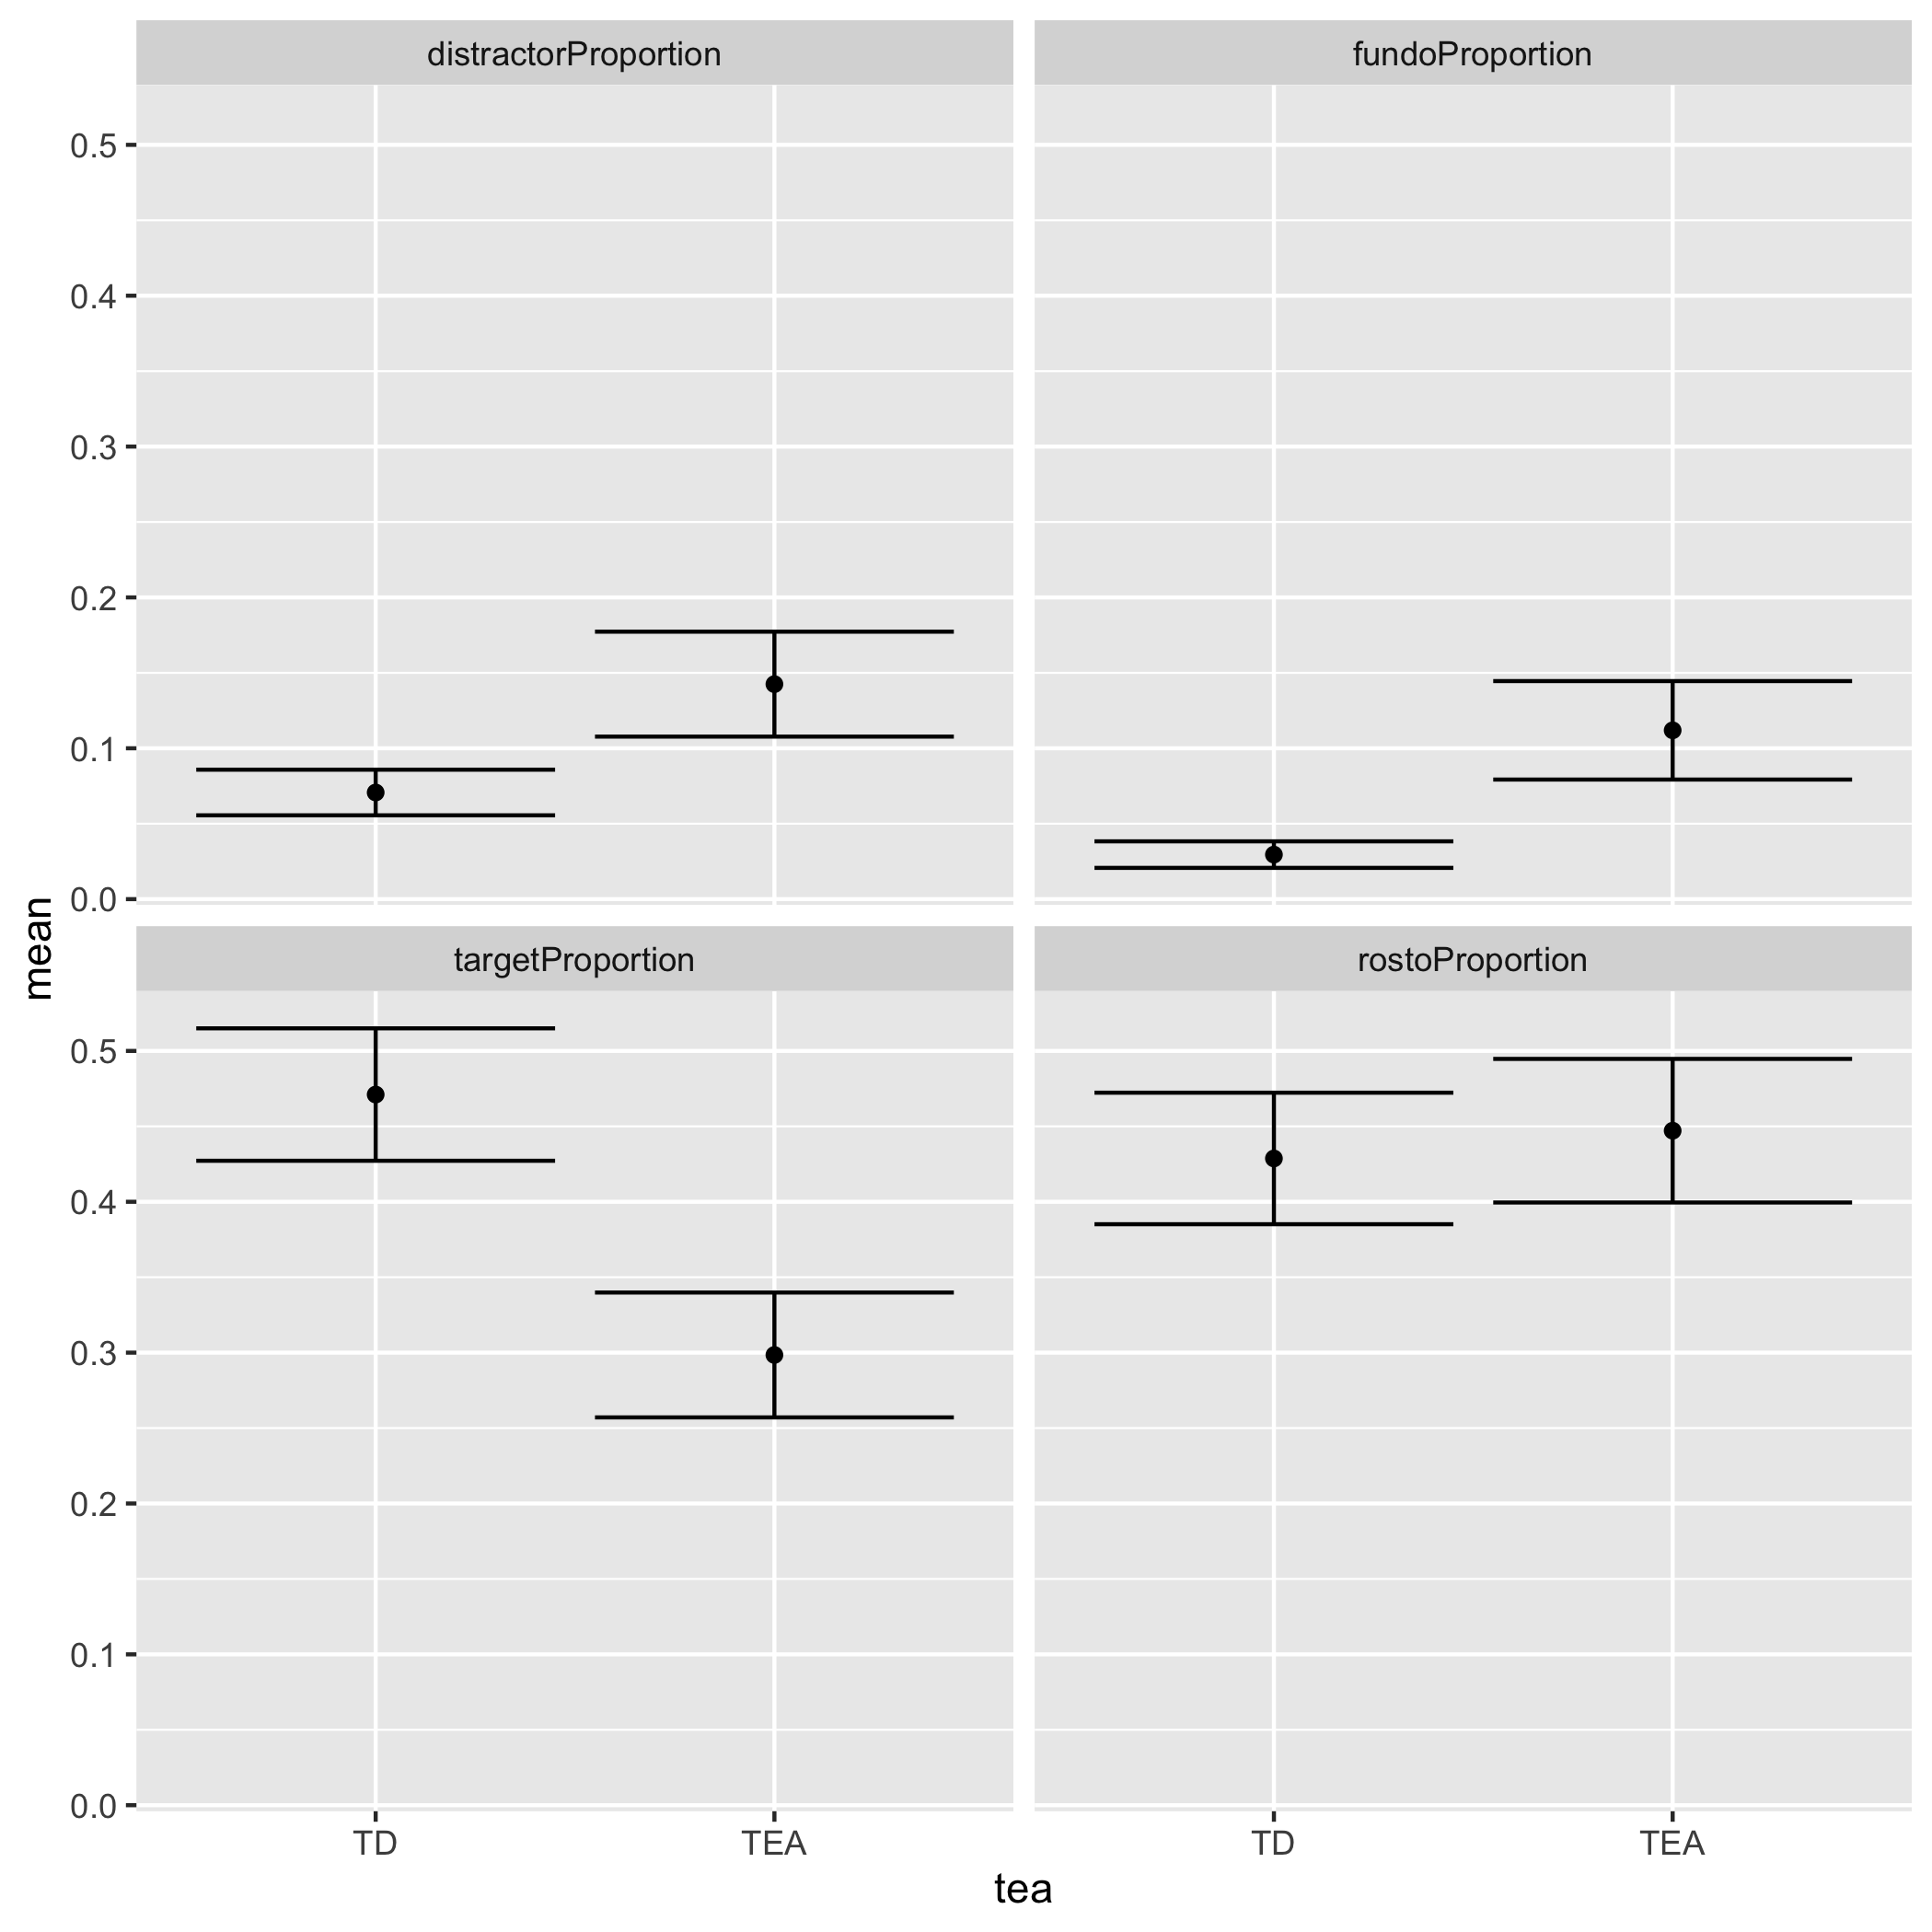
\includegraphics[scale=0.2]{./teaVariableProportion.png}}
  \centering
\end{figure}

Ho, D., Imai, K., King, G., \& Stuart, E. A. (2011). MatchIt: Nonparametric Preprocessing for Parametric Causal Inference. Journal of Statistical Software, 42(8), 1–28. https://doi.org/10.18637/jss.v042.i08

\end{document}
